%%%%%%%%%%%%%%%%%%%%%%%%%%%%%%%%%%%%%%%%%%%%%%%%%%%%%%%%%%%%%%%%%%%%
\begin{frame} 
\frametitle{История развития региона}
\begin{wrapfigure}{l}{0.5\linewidth}
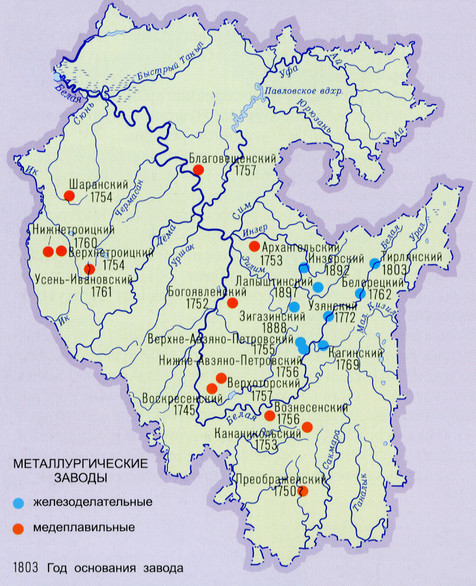
\includegraphics[width=1\linewidth]{pics/sasha/factories_18-19} 
\end{wrapfigure}
Присоединение территорий республики завершилось к середине XVII века. \\[10pt]

Вторая половина XVII -- массовые восстания. 1773-1775 гг -- Крестьянская война. \\[10pt]

Со второй половины XVIII века начинают сооружаться заводы. \\[10pt]

20 марта 1919 г. -- создана Башкирская Автономная Советская Республика. Во время Гражданской войны экономика республики претерпела серьезный урон: объем производства промышленности упал на 70\% и восстановился лишь к 1926 году.

\end{frame}
%%%%%%%%%%%%%%%%%%%%%%%%%%%%%%%%%%%%%%%%%%%%%%%%%%%%%%%%%%%%%%%%%%%%

%%%%%%%%%%%%%%%%%%%%%%%%%%%%%%%%%%%%%%%%%%%%%%%%%%%%%%%%%%%%%%%%%%%%
\begin{frame}
\frametitle{История развития региона}

В 1920-30-е годы -- рост промышленного производства. 1932 г. -- начало нефтедобывающей промышленности Башкортостана. Темпы роста:
\begin{center}
\begin{tabular}{|c|c|c|c|c|c|c|c|}
\hline 
Год & 1913 & 1940 & 1950 & 1960 & 1970 & 1980 & 1990 \\ 
\hline 
\% & 1,0 & 10 & 41 & 186 & 478 & 983 & 1221 \\ 
\hline 
\end{tabular} 
\end{center}

Во время Великой Отечественной войны Башкортостан стал одним из важнейших регионов перебазирования промышленности страны.\\[5pt]

После войны республика стала ведущим регионом по нефтепереработке, а по добыче нефти занимает второе место в СССР. В 1966-1980 гг. в БАССР были запущены 832 предприятия. Промышленно-производственные фонды выросли в 2,8 раза, выпуск продукции – в 2,4 раза. 

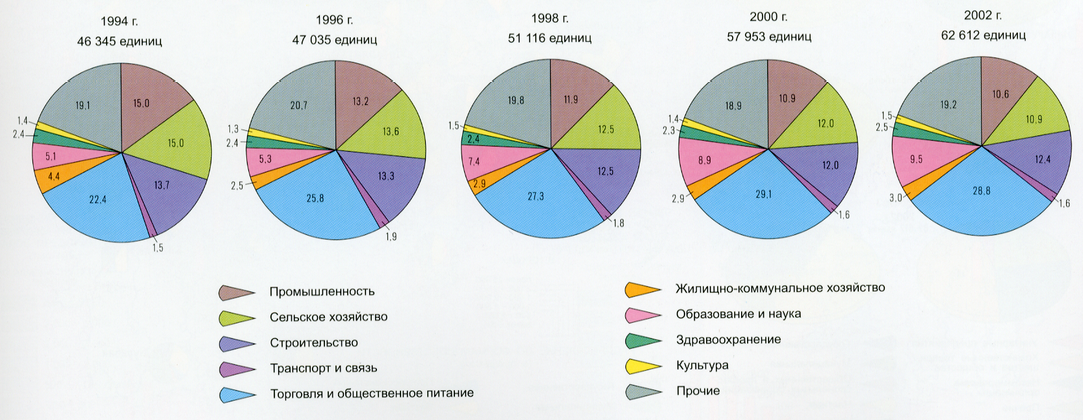
\includegraphics[width=1\linewidth]{pics/sasha/industries}
Распределение предприятий и организаций Башкортостана по отраслям (\%)

\end{frame}
%%%%%%%%%%%%%%%%%%%%%%%%%%%%%%%%%%%%%%%%%%%%%%%%%%%%%%%%%%%%%%%%%%%%

%%%%%%%%%%%%%%%%%%%%%%%%%%%%%%%%%%%%%%%%%%%%%%%%%%%%%%%%%%%%%%%%%%%%
\begin{frame}
\frametitle{Отраслевая и территориальная структура экономики}

\begin{wrapfigure}{r}{0.4\linewidth}
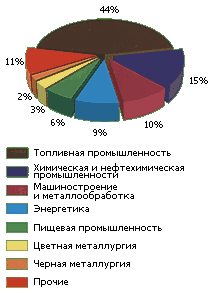
\includegraphics[width=1\linewidth]{pics/sasha/promstruct}
\end{wrapfigure}
Центры промышленного производства: \\[10pt]
\begin{itemize}
\item Уфа \\[10pt] 
\item Стерлитамак \\[10pt]
\item Салават \\[10pt]
\item Ишимбай \\[10pt]
\item Нефтекамск 
\end{itemize}
\vfill
На предприятиях этих городов производится более половины объёма всей промышленной продукции Башкортостана.

\end{frame}
%%%%%%%%%%%%%%%%%%%%%%%%%%%%%%%%%%%%%%%%%%%%%%%%%%%%%%%%%%%%%%%%%%%%

%%%%%%%%%%%%%%%%%%%%%%%%%%%%%%%%%%%%%%%%%%%%%%%%%%%%%%%%%%%%%%%%%%%%
\begin{frame}
\frametitle{Нефтедобыча и нефтехимическая промышленность}

В республике разведано 191 месторождение нефти и газа, из них в разработке находится 161 месторождение.  \\[10pt]

Ведущее нефтегазодобывающее предприятие Башкирии — ПАО «Акционерная нефтяная компания „Башнефть“», на долю которого приходится более 98\% объёма нефтедобычи и практически весь объём добываемого газа. \\[10pt]

Ведущие предприятия:
\begin{itemize}
\item г. Уфа: «Башнефть-Уфанефтехим», «Башнефть-УНПЗ» и «Башнефть-Новойл»; ОАО «Уфаоргсинтез»
\item г. Салават: ОАО «Газпром нефтехим Салават»
\item г. Стерлитамак: ОАО «Стерлитамакский нефтехимический завод»; ОАО «Башкирская содовая компания»
\end{itemize}

\end{frame}
%%%%%%%%%%%%%%%%%%%%%%%%%%%%%%%%%%%%%%%%%%%%%%%%%%%%%%%%%%%%%%%%%%%%

%%%%%%%%%%%%%%%%%%%%%%%%%%%%%%%%%%%%%%%%%%%%%%%%%%%%%%%%%%%%%%%%%%%%
\begin{frame}
\frametitle{Нефтедобыча и нефтехимическая промышленность}


\end{frame}
%%%%%%%%%%%%%%%%%%%%%%%%%%%%%%%%%%%%%%%%%%%%%%%%%%%%%%%%%%%%%%%%%%%%

%%%%%%%%%%%%%%%%%%%%%%%%%%%%%%%%%%%%%%%%%%%%%%%%%%%%%%%%%%%%%%%%%%%%
\begin{frame}
\frametitle{Нефтедобыча и нефтехимическая промышленность}


\end{frame}
%%%%%%%%%%%%%%%%%%%%%%%%%%%%%%%%%%%%%%%%%%%%%%%%%%%%%%%%%%%%%%%%%%%%

%%%%%%%%%%%%%%%%%%%%%%%%%%%%%%%%%%%%%%%%%%%%%%%%%%%%%%%%%%%%%%%%%%%%
\begin{frame}
\frametitle{Нефтедобыча и нефтехимическая промышленность}


\end{frame}
%%%%%%%%%%%%%%%%%%%%%%%%%%%%%%%%%%%%%%%%%%%%%%%%%%%%%%%%%%%%%%%%%%%%

%%%%%%%%%%%%%%%%%%%%%%%%%%%%%%%%%%%%%%%%%%%%%%%%%%%%%%%%%%%%%%%%%%%%
\begin{frame}
\frametitle{Нефтедобыча и нефтехимическая промышленность}


\end{frame}
%%%%%%%%%%%%%%%%%%%%%%%%%%%%%%%%%%%%%%%%%%%%%%%%%%%%%%%%%%%%%%%%%%%%

%%%%%%%%%%%%%%%%%%%%%%%%%%%%%%%%%%%%%%%%%%%%%%%%%%%%%%%%%%%%%%%%%%%%
\begin{frame}
\frametitle{Нефтедобыча и нефтехимическая промышленность}


\end{frame}
%%%%%%%%%%%%%%%%%%%%%%%%%%%%%%%%%%%%%%%%%%%%%%%%%%%%%%%%%%%%%%%%%%%%

%%%%%%%%%%%%%%%%%%%%%%%%%%%%%%%%%%%%%%%%%%%%%%%%%%%%%%%%%%%%%%%%%%%%
\begin{frame}
\frametitle{Нефтедобыча и нефтехимическая промышленность}


\end{frame}
%%%%%%%%%%%%%%%%%%%%%%%%%%%%%%%%%%%%%%%%%%%%%%%%%%%%%%%%%%%%%%%%%%%%

%%%%%%%%%%%%%%%%%%%%%%%%%%%%%%%%%%%%%%%%%%%%%%%%%%%%%%%%%%%%%%%%%%%%
\begin{frame}
\frametitle{Отраслевая и территориальная структура экономики}


\end{frame}
%%%%%%%%%%%%%%%%%%%%%%%%%%%%%%%%%%%%%%%%%%%%%%%%%%%%%%%%%%%%%%%%%%%%